\chapter{Conceptual Design}
\label{sec:design}
%
\todo{Describe Chapter}


% ===========================================
% ===========================================
\section{Cluster Architecture}

\begin{figure}[h]%
\centering
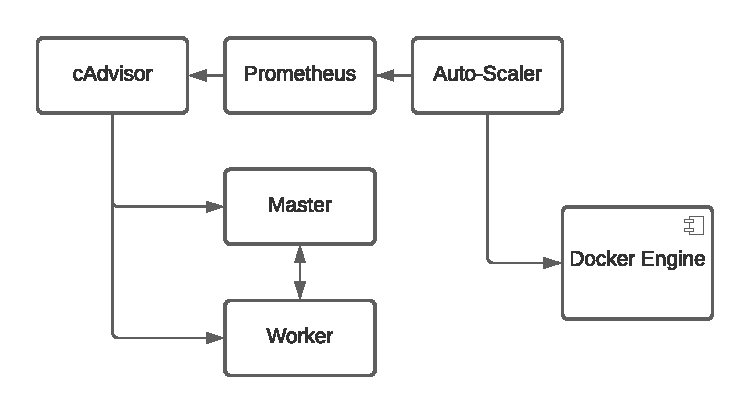
\includegraphics[scale=0.8]{images/04_conceptual_design/cluster_architecture/overall_architecture}%
\caption{Scaling process UML activity model - Source: Authors own model.}%
\label{fig:ca-overall_architecture}%
\end{figure}

% Components
The cluster consists of two main parts, the Autonomic Manager and the Apache Spark cluster. The autonomic manager consists of three components, cAdvisor for collecting metrics from all running Docker container, Prometheus to store metrics and the auto-scaler to scale the number of Spark worker according to the workload.
The Apache Spark cluster is the computing environment, consisting of one Apache Spark master and a dynamic number of Apache Spark worker. A Spark-Submit component which will deployed if a Spark application gets executed in the cluster.
Each component is supposed to be a Docker container running on the same host. The autonomic manager and the Apache Spark cluster have its own Docker network.
% Communication
The autonomic manager and the Apache Spark cluster don't communicate between each other.The autonomic manager gets its metrics directly from the Docker engine and sends instructions to the Docker engine to scale the number of Spark worker.


% ===========================================
% ===========================================
\section{Apache Spark Cluster}
% Hier Bild nur von Apache Spark Cluster, etwas detailierter
The Apache Spark cluster is responsible to execute the computing application. It consists of one Apache Spark Master and a dynamic number of Apache Spark Worker. To create a Apache Saprk cluster, the master and all worker are deployed in standalone mode (described in section XY).
All Spark components run in a single isolated Docker network.


\subsection{Computing Environment}
Computing environment consists only of Apache Spark Master and Spark worker. All Spark components are deplyed in standalone mode and each is a single container in the same Docker network. The Apache Spark master distributed the workload of an application across all available spark worker.

\subsection{Spark Submit}
Spark submit is a single component in the APache Spark cluster. It is a Apache Spark submit runtime running in a single Docker container. Whenever a Saprk application needs to be executed, a Spark submit container gets deployed in the Apache Saprk and submits the application to the Spark master. After completion, the Spark submit container gets removed automatically.


% ===========================================
% ===========================================
\section{Autonomic Manager}
% Short description of old section
The autonomic manager is implemented according to the MAPE architecture (introduced in SECTION AB). It is responsible to monitor the CPU and GPU utilization of all running Spark Worker and dynamically scales the number of Spark worker based on the observed metrics. As illustrated in \Fig{fig:ca-overall_architecture}, the autonomic manager consists of three components to compose an autonomic manager.


\subsection{Workflow}
% Process figure
\begin{figure}[h]%
\centering
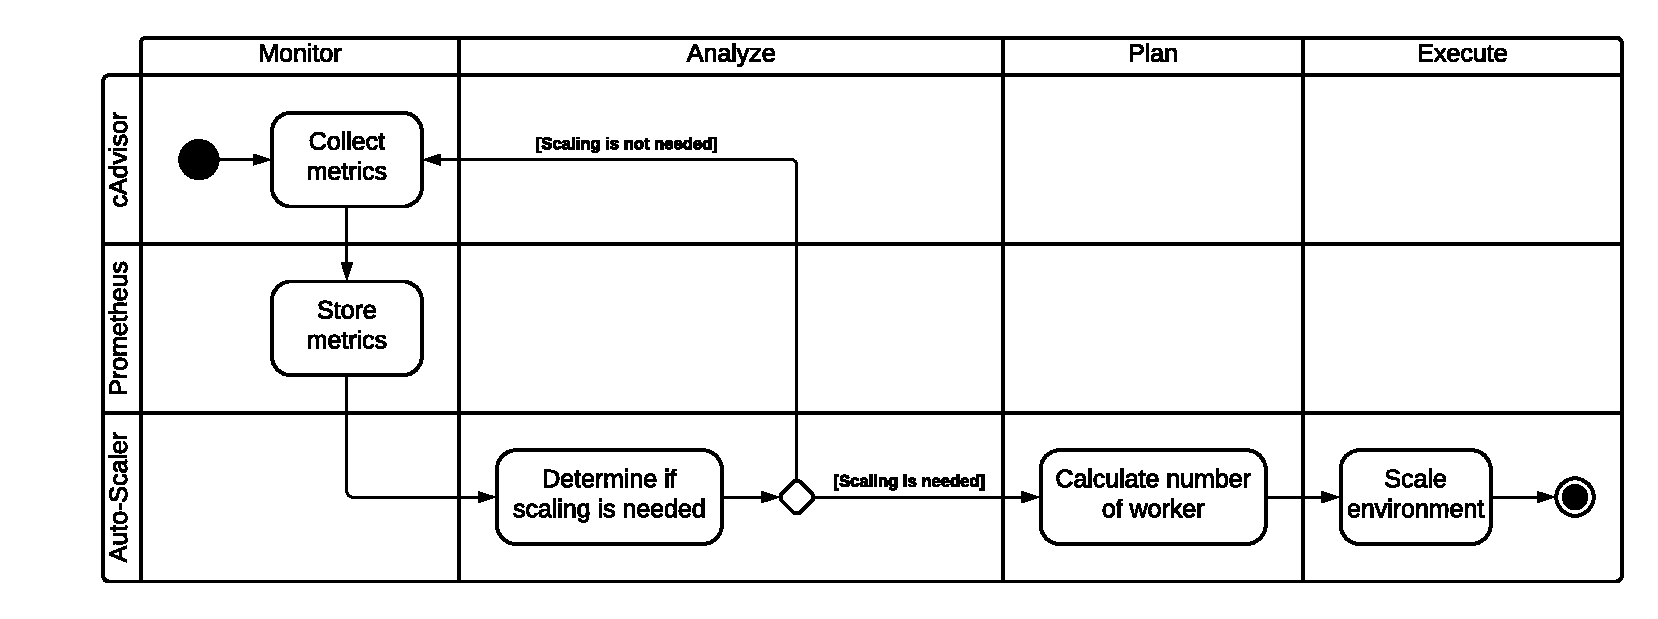
\includegraphics[scale=0.65]{images/04_conceptual_design/autonomic_manager/autonomic_manager_workflow}%
\caption{Scaling process UML activity model - Source: Authors own model.}%
\label{fig:am-workflow}%
\end{figure}

% Short description
As illustrated in \Fig{fig:am-workflow}, the workflow of the autonomic manager is implemented as a loop. In each iteration, the autonomic manager collects and analyzes related metrics. If needed, the autonomic manager will create a scaling plan and execute it in the end of an iteration.


% How is the workflow structured
Following, each step is described in detail:

\begin{enumerate}
\item \textbf{Collect metrics:} CPU and GPU metrics need to be collected from the Docker engine. The collected data needs to be filtered aggregated.
\item \textbf{Analyze metrics:} Collected metrics need to be analyzed to determine if a scaling action is need. If the computing environment runs smoothly and no scaling action is needed, the first two steps will be repeated until a scaling action is necessary.
\item \textbf{Create scaling plan:} If the computing environment has to be scaled, a scaling plan will be generated. The scaling plan consists of instructions how many Spark worker have to added or removed.
\item \textbf{Execute scaling plan:} The created scaling plan will be executed to accommodate the performance goals of the environment.
\end{enumerate}


\subsection{Design}

% Component design
\begin{figure}[h]%
\centering
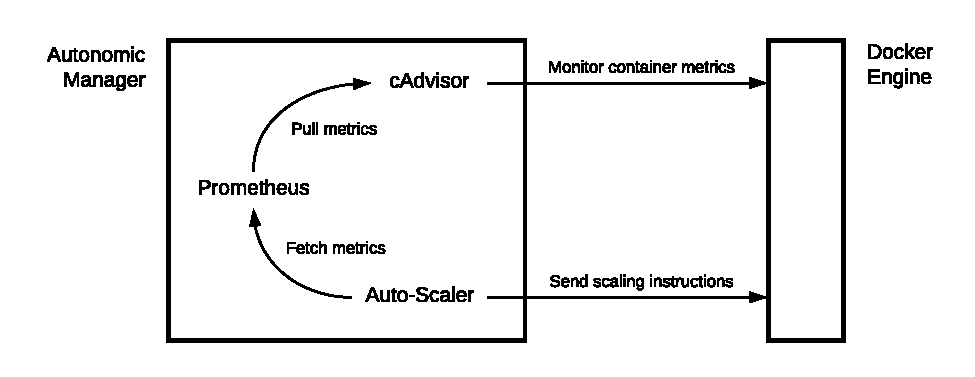
\includegraphics[scale=0.85]{images/04_conceptual_design/autonomic_manager/autonomic_manager_overview}%
\caption{Scaling process UML activity model - Source: Authors own model.}%
\label{fig:am-design-component}%
\end{figure}

The autonomic manager consists of three different components: cAdvisor, Prometheus, Auto-Scaler. Each components has a different responsibility. 


% cAdvisor
cAdvisor constantly monitors all Docker containers in the environment and makes perormance and system metrics available via its API.
% Prometheus
Prometheus pulls the metrics from cAdvisor. The metrics can be filtered and aggregated via Prometheus PromQL language. In addition, Prometheus stores metrics as time-series data in its database.
% Monitor phase
cAdvisor and Prometheus perform the monitor phase of the MAPE architecture.


% Auto-Scaler
The Auto-Scaler is responsible for the analyze, plan and execute phase. Each interval, the Auto-Scaler obtains the CPU and GPU metrics from the Prometheus API. It analyzes the metrics to determine if a scaling action is needed and creates and executes a scaling plan.


% All are Docker container
Each component of the autonomic manager is supposed to execute in an individual Docker container. To establish an isolated communication across all three components, all Docker container run in a single Docker network which is exclusively for the autonomic manager.


\section{Auto-Scaler}
% What is the Auto-Scaler
The Auto-Scaler is a component of the the Autonomic Manager and is responsible for the Analyze, Plan and Execution phase.
% Complete autonomic manager
Together with cAdvisor and Prometheus, the Auto-Scaler builds a complete Autonomic Manager according to the architecture demonstrated in \SubSec{subsec:background-autonomic_computing-autonomic_manager}.
% controll loop
In addition, the Auto-Scaler implements the control-loop which is responsible to make adjustments in the environment.
% Communication
Since Prometheus collects and stores available metrics from cAdvisor, the Auto-Scaler has not to communicate with cAdvisor.

% HIER NOCH BILD VON SCALER WIE MIT DER MAPE ARCH


\subsection{Configuration}
\label{subsec:design-auto_scaler-configuration}
The Auto-Scaler needs specific configuration properties to be able to collect the correct metrics from Prometheus and deploy new Apache Spark worker container in the environment. The following are properties that have to be defined to ensure that the Auto-Scaler is able to collect meaningful metrics and scale Apache Spark worker as expected.

\subsubsection{General properties}

\begin{itemize}
\item \textbf{Interval seconds:} The number of seconds when the loop has to repeat needs to be defined.
\end{itemize}

\subsubsection{Utilization thresholds}

\begin{itemize}
\item \textbf{CPU/GPU utilization thresholds:} To determine if a scaling action is needed, the scaling heat algorithm needs the minimum and maximum CPU/GPU utilization defined by an administrator.
\end{itemize}

\subsubsection{Apache Spark worker properties}

\begin{itemize}
\item \textbf{Worker image:} To guarantee that each Spark worker is homogeneous, all worker container should be created with the same image.

\item \textbf{Worker network:} To establish communication between all Spark worker and the Spark master, all new Spark worker container should be in the same network.

\item \textbf{Worker thresholds:} The minimum and maximum number of concurrent Spark worker should be defined. To avoid the cold start effect, the minimum amount of worker should be 1. \todo{CHeck nochmal den Cold Start effekt}

\item \textbf{Apache Spark master URI:} To distribute the workload across all Spark Worker, all Spark Worker need to communicate with the Spark master.
\end{itemize}

\subsubsection{Prometheus properties}

\begin{itemize}
\item \textbf{Prometheus URL:} The Auto-Scaler will collect the configured metrics from Prometheus REST API.

\item \textbf{Prometheus query:} A PromQL query needs to be defined to collect specific metrics for CPU utilization calculation. 
\end{itemize}


\subsection{Analyze}
% Short intro to analyze phase
In order to determine if a scaling-action is necessary, the Auto-Scaler has to analyze the collected metrics. 
% How to analyze
During each period, the Auto-scaler queries the time-series database from Prometheus with the configured query to get the CPU and GPU utilization metrics. The configured query will be send to the Prometheus API.
% Determine if scaling is needed
After the metrics are received, the Auto-Scaler determines if a scaling action is needed using the Scaling Heat algorithm (introduced in Section AB). If scaling is not necessary, the Auto-Scaler continues to collect metrics from Prometheus.

\subsection{Plan}
% Short intro
If a scaling-action is necessary, the Auto-Scaler will create a scaling plan to accommodate the defined goals and objectives.

A scaling plan consists of instructions to add or remove Spark worker which will be send to the Docker engine.

To determine how many Spark worker needs to be added, the Auto-Scaler uses the KHPA algorithm (introduced in Section BC). Before a scaling plan will be executed, the Auto-Scaler needs to check the maximum limit of Spark worker to prevent an overflow.

% Downscaling 
% Cooldown phase

% Goals
The goals and objectives which need to be achieved, are defined in the Auto-Scaler configuration (described in \SubSec{subsec:design-auto_scaler-configuration}).
% MinMax CPU GPU utilization
The percentage of minimum and maximum CPU and GPU utilization across all Spark worker have to defined (described in \SubSec{subsec:design-auto_scaler-configuration}). These are the goals that the Auto-Scaler tries to achieve.
% MinMax Spark Worker
In addition, the minimum and maximum amount of concurrent Spark Worker have to be set (described in \SubSec{subsec:design-auto_scaler-configuration}) to guarantee that not too many or less Spark Worker are running at the same time HIER IST SEHR SCHWAMMIG; GUCK MAL IN DIE PAPER.
%
To achieve the defined goals of CPU and GPU utilization as well as ensure that the minimum and maximum number of concurrent Spark worker is observed, the Auto-Scaler will use the KHPA algorithm (described in Section BLA).


% ===========================================
% ===========================================
\section{Metrics}
% Welche metrics gibt es
% Welche metrics werden gesammelt (nur von den Worker)
% Wie werden die metrics berechnet

\subsection{CPU Utilization}
% Evtl ist hier der faösche platz -> Besser eine Metrics section wo erklärt wird, wie das berechnet werden soll.
\todo{Hier auf Tabelle verweisen (Anhang) Metriken die von Prometheus + cAdvisor bereitgestellt werden}

% How is the CPU Utilization being calculated
To adapt to business needs, the CPU percentage of each Spark Worker will be calculated. Prometheus provides several metrics to calculate the CPU percentage. The CPU percentage of all Worker can be calculated as follows:

\begin{equation}
CPUUtilization = \dfrac{\sum SparkWorkerCPUUtilization}{NumberOfSparkWorker}
\label{eq:formel}
\end{equation}


\subsection{GPU Utilization}

\begin{equation}
GPUUtilization = \dfrac{\sum SparkWorkerGPUUtilization}{NumberOfSparkWorker}
\label{eq:formel}
\end{equation}

